\documentclass[11pt]{article}
\usepackage[scaled=0.92]{helvet}
\usepackage{geometry}
\geometry{letterpaper,tmargin=1in,bmargin=1in,lmargin=1in,rmargin=1in}
\usepackage[parfill]{parskip} % Activate to begin paragraphs with an empty line rather than an indent %\usepackage{graphicx}
\usepackage{amsmath,amssymb, mathrsfs, dsfont}
\usepackage{tabularx}
\usepackage[font=footnotesize,labelfont=bf]{caption}
\usepackage{graphicx}
\usepackage{xcolor}
%\usepackage[linkbordercolor ={1 1 1} ]{hyperref}
%\usepackage[sf]{titlesec}

\usepackage{../report}

\begin{document}
\title{Heuristic Analysis}
\author{ Tianpei Xie}
\date{ Nov. 25th., 2017 }
\maketitle
\section{Heuristics}
In the submitted codes, I includes two heuristics  and the final main $custom\_score$ function is a combination of two of them.

\begin{itemize}
\item $custom\_score\_2$ implements the center heuristic. It computes the distance between a move and the center of the board. The intuition is that the possible move at center of the board is largest, thus is most beneficial. 

\item $custom\_score\_3$ implements a modified version of $open_moves$, which computes the difference between all possible moves for current player and all possible moves of its opponent. In this implementation, we put more weights on the opponents possible moves so that  the agent will be more aggressive. 

\item $custom\_score$ combines both heuristic to have a better performance than either.  It is seen that against \emph{AB$\_$Improved}, the proposed \emph{AB$\_$Custom} win with about $62\% - 66\%$ of chance. Compared with the\emph{ AB$\_$improved } which uses a direct difference between the size of possible moves for current player with all possible moves of its opponent, we put more weights on minimizing the possible move of its opponents, which makes the agent more aggressive to block the opponent. This contributes to a slightly better chance of winning for the proposed solution. 

The included is the score from the tournament (with no. of matches $=5$)
\begin{figure}[htb] 
\begin{minipage}[b]{0.48\linewidth}
  \centering
  \centerline{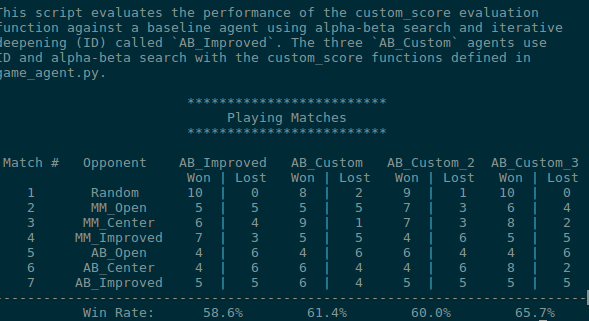
\includegraphics[scale=0.35]{result_1.png}}
  \centerline{\footnotesize{(a)}}
\end{minipage}
\hfill
\begin{minipage}[b]{0.48\linewidth}
  \centering
  \centerline{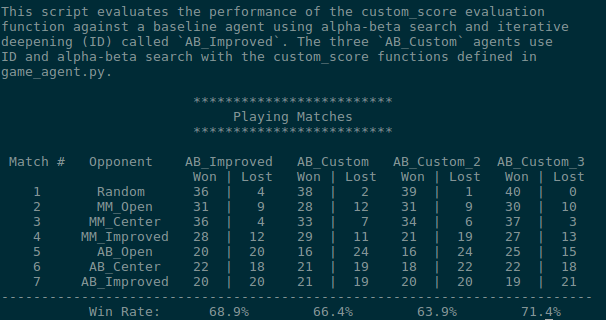
\includegraphics[scale=0.35]{result_3.png}}
 \centerline{\footnotesize{(b) }}
\end{minipage}\vspace{-10pt}
\caption{(a) Run with $5$ matches each (b) Run with $20$ matches each. }
%\caption{ (a) Test error ($\%$) vs. noise level $R$ (corruption rate $=0.2$). (b) Test error ($\%$) vs. corruption rate ($R=55$) on simulated data.}
\label{fig:pred-acc}
\end{figure}
%\begin{figure}[htb] 
%\begin{minipage}[h]{0.4 \linewidth}
%  \centering
%  \centerline{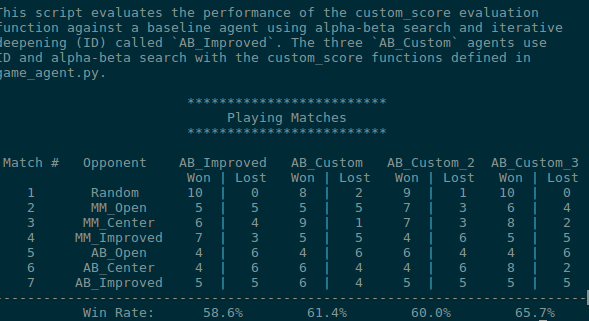
\includegraphics[scale = 0.35]{./result_1.png}}\,
%  \end{minipage}
%  \begin{minipage}
%  \centerline{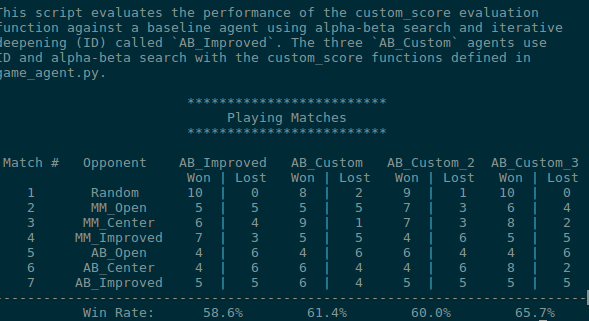
\includegraphics[scale = 0.35]{./result_1.png}}
%    \end{minipage}
%  \caption{\scriptsize{\textbf{Running result }}} \label{fig: person_network}
%\end{figure}
\end{itemize}

As shown above, we recommend using a \emph{combination} of modified $open\_move$ and $center\_heuristic$ as an evaluation function. It has the following benefits
\begin{enumerate}
\item Both $open\_move$ and $center\_heuristic$ are easy to compute, with fast implementation avaiable. It allows the algorithm to handle large scale problem effectively. 
\item The modified $open\_move$ emphasize the aggressive strategy to actively block the opponents, we can also add defensive version by adding more weights on the possible self-moves. It effective goes against the simple $open\_move$ strategy.
\item The final custom function is a linear combination of both strategies. Note that the weight may not need to be fixed. Allowing adjustable weight make it possible to \emph{learn} an ensemble of value functions, similar to what used in the AlphaGo model. It provides a general strategy that not only fit this game but allows for further varities of value functions to be used adaptively. 
\end{enumerate}

\end{document}